\documentclass{article}   

\usepackage{geometry}
\usepackage{qtree}
\usepackage[square,numbers]{natbib}
% \usepackage{cite}  
\geometry{a4paper}

\usepackage[]{algorithm2e}
\usepackage{amsthm}
\newtheorem{theorem}{Theorem}[section]
\newtheorem{corollary}{Corollary}[theorem]
\newtheorem{lemma}[theorem]{Lemma}

\usepackage[utf8]{inputenc}
\usepackage[T1]{fontenc}    % use 8-bit T1 fonts
\usepackage{lmodern}
\usepackage{hyperref}       % hyperlinks
\usepackage{lipsum}

\usepackage{color, colortbl}

\definecolor{Gray}{gray}{0.9}

\usepackage[protrusion=true,expansion=true]{microtype}

\usepackage{amssymb}
\usepackage{amsfonts}
\usepackage{eqnarray,amsmath}
\usepackage[table]{xcolor}

\usepackage{listings}
\usepackage{graphicx}
\usepackage{dirtytalk}

\usepackage[table]{xcolor}
\usepackage{rotating}
\usepackage{caption}

%% if you use PostScript figures in your article
%% use the graphics package for simple commands
\usepackage{graphics}


%% or use the graphicx package for more complicated commands
\usepackage{graphicx}
\usepackage[table]{xcolor}

\usepackage{indentfirst}
\usepackage[utf8]{inputenc}
 \usepackage{subcaption}
\usepackage{listings}
\usepackage{xcolor}
 
\definecolor{codegreen}{rgb}{0,0.6,0}
\definecolor{codegray}{rgb}{0.5,0.5,0.5}
\definecolor{codepurple}{rgb}{0.58,0,0.82}
\definecolor{backcolour}{rgb}{0.95,0.95,0.92}
 
\lstdefinestyle{mystyle}{
    backgroundcolor=\color{backcolour},   
    commentstyle=\color{codegreen},
    keywordstyle=\color{magenta},
    numberstyle=\tiny\color{codegray},
    stringstyle=\color{codepurple},
    basicstyle=\ttfamily\footnotesize,
    breakatwhitespace=false,         
    breaklines=true,                 
    captionpos=b,                    
    keepspaces=true,                 
    numbers=left,                    
    numbersep=5pt,                  
    showspaces=false,                
    showstringspaces=false,
    showtabs=false,                  
    tabsize=2
}
%https://tex.stackexchange.com/questions/96825/nicely-formatted-where-statement-for-maths
 \newenvironment{where}{\noindent{}where\begin{itemize}}{\end{itemize}}
 
 
\lstset{style=mystyle}
% please place your own definitions here and don't use \def but
% \newcommand{}{}
%
% Insert the name of "your journal" with
% \journalname{myjournal}
%
\begin{document}

\title{%
  Practice 4: The Poisson distribution} %\\~\\
  %\Large }
\author{Mayra Cristina Berrones Reyes 6291}

\maketitle

\section{Introduction}

For this practice, we explore the properties of several \texttt{R} distributions, such as \texttt{rpois, runif,} and \texttt{rexp}, taking note in their difference as well as the similarities under certain circumstances. Before beginning with any experimentation, a brief description of each distribution will assist in the understanding of the problem.\\

\subsection{Poisson distribution}

A Poisson random variable can be used to model the number of times an event happened in a certain interval of time. It is described in terms of the rate in which this events happen, because an event can occur several times in a single interval. To be able to use this distribution we have to know the average number of events in an interval, which is designated by the sign of lambda ($\lambda$) \cite{poison}.\\

Lambda is also called the rate parameter. The probability of k events happening in an interval is represented in Equation \ref{eq1}:

\begin{equation} \label{eq1}
P(k \mbox{ events in interval}) = e^{-\lambda}\frac{\lambda^k}{k!}
\end{equation}

\smallskip

In \texttt{R} we can generate this distribution with the module \texttt{rpois}. The description for this module in \texttt{R help} says that is a \say{Density, distribution function, quantile function and random generation for the Poisson distribution with parameter $\lambda$} \cite{rpois}. The parameters it takes are stated in Equation \ref{eq2}:

\begin{equation} \label{eq2}
\mbox{\texttt{rpois}(n, lambda)}
\end{equation}

\begin{where}
\item \textbf{n} is the number of random values to return.
\item \textbf{lambda} is the vector of non negative means.
\end{where}

\smallskip

\subsection{Exponential distribution}

The exponential distribution describes the time between events in a process in which they occur in a continuous and independent manner at a constant average rate. This distribution also uses the parameter lambda ($\lambda$) and it is called the rate parameter \cite{distributions}. The equation for this distribution can be seen in Equation \ref{eq3}:

\begin{equation} \label{eq3}
f(x;\lambda) = 
  \begin{cases} 
   \lambda \exp^{-\lambda x} & \text{if } x \geq 0 \\
   0       & \text{if } x < 0
  \end{cases}
\end{equation}

\smallskip

In \texttt{R} we can generate this distribution with the module \texttt{rexp}. The description for this module in \texttt{R help} says that is a \say{Density, distribution function, quantile function and random
     generation for the exponential distribution with rate (i.e., mean 1/rate)} \cite{rexp}. This is a very important distinction, because we do not have to make the division in the variable ourselves, only add the \textit{rate} value as it is \cite{distributions}.\\ 

The parameters it takes are stated in Equation \ref{eq4}:

\begin{equation} \label{eq4}
\mbox{\texttt{rexp}(n, rate = 1)}
\end{equation}

\begin{where}
\item \textbf{n} is the number of observations. If length(n) $>$ 1, the length is taken to be the number required.
\item \textbf{rate} is the vector of rates.
\end{where}

\smallskip

\subsection{Uniform distribution}

The uniform distribution is one of the most simple and commonly used distribution. In the continuous uniform distribution we have the probability in Equation \ref{eq5} as:

\begin{equation} \label{eq5}
f(x) = 
  \begin{cases} 
   \frac{1}{b-a}  & \text{for } a \leq x \leq b \\
   0       & \text{for } x < a \mbox{ or } x > b 
  \end{cases}
\end{equation}

In this distribution, any interval of numbers of equal width have an equal probability of being observed. The curve describing the distribution is a rectangle with a constant height across interval and 0 height elsewhere. We can use in \texttt{R} a tool to see the this distribution, called \texttt{runif}. The description for this module in \texttt{R help} says that \say{These functions provide information about the uniform distribution on the interval from \texttt{min} to \texttt{max}. \texttt{runif} generates random deviates} \cite{runif}.\\

The parameters it takes are stated in Equation \ref{eq6}:

\begin{equation} \label{eq6}
\mbox{\texttt{runif}(n, min = 0, max = 1)}
\end{equation}

\begin{where}
\item \textbf{n} is the number of observations. If length(n) $>$ 1, the length is taken to be the number required.
\item \textbf{min, max} are the lower and upper limits of the distribution. Must be finite.
\end{where}


\section{Comparisons between distributions}

In Figure \ref{fig1} we can appreciate how all of the described distributions behave. None of them look similar to one another. The goal of this practice is to show with which parameters we can make all of this distributions look similar, and explain why that is possible.\\

\begin{figure}[]
\begin{subfigure}{.33\textwidth}
  \centering
  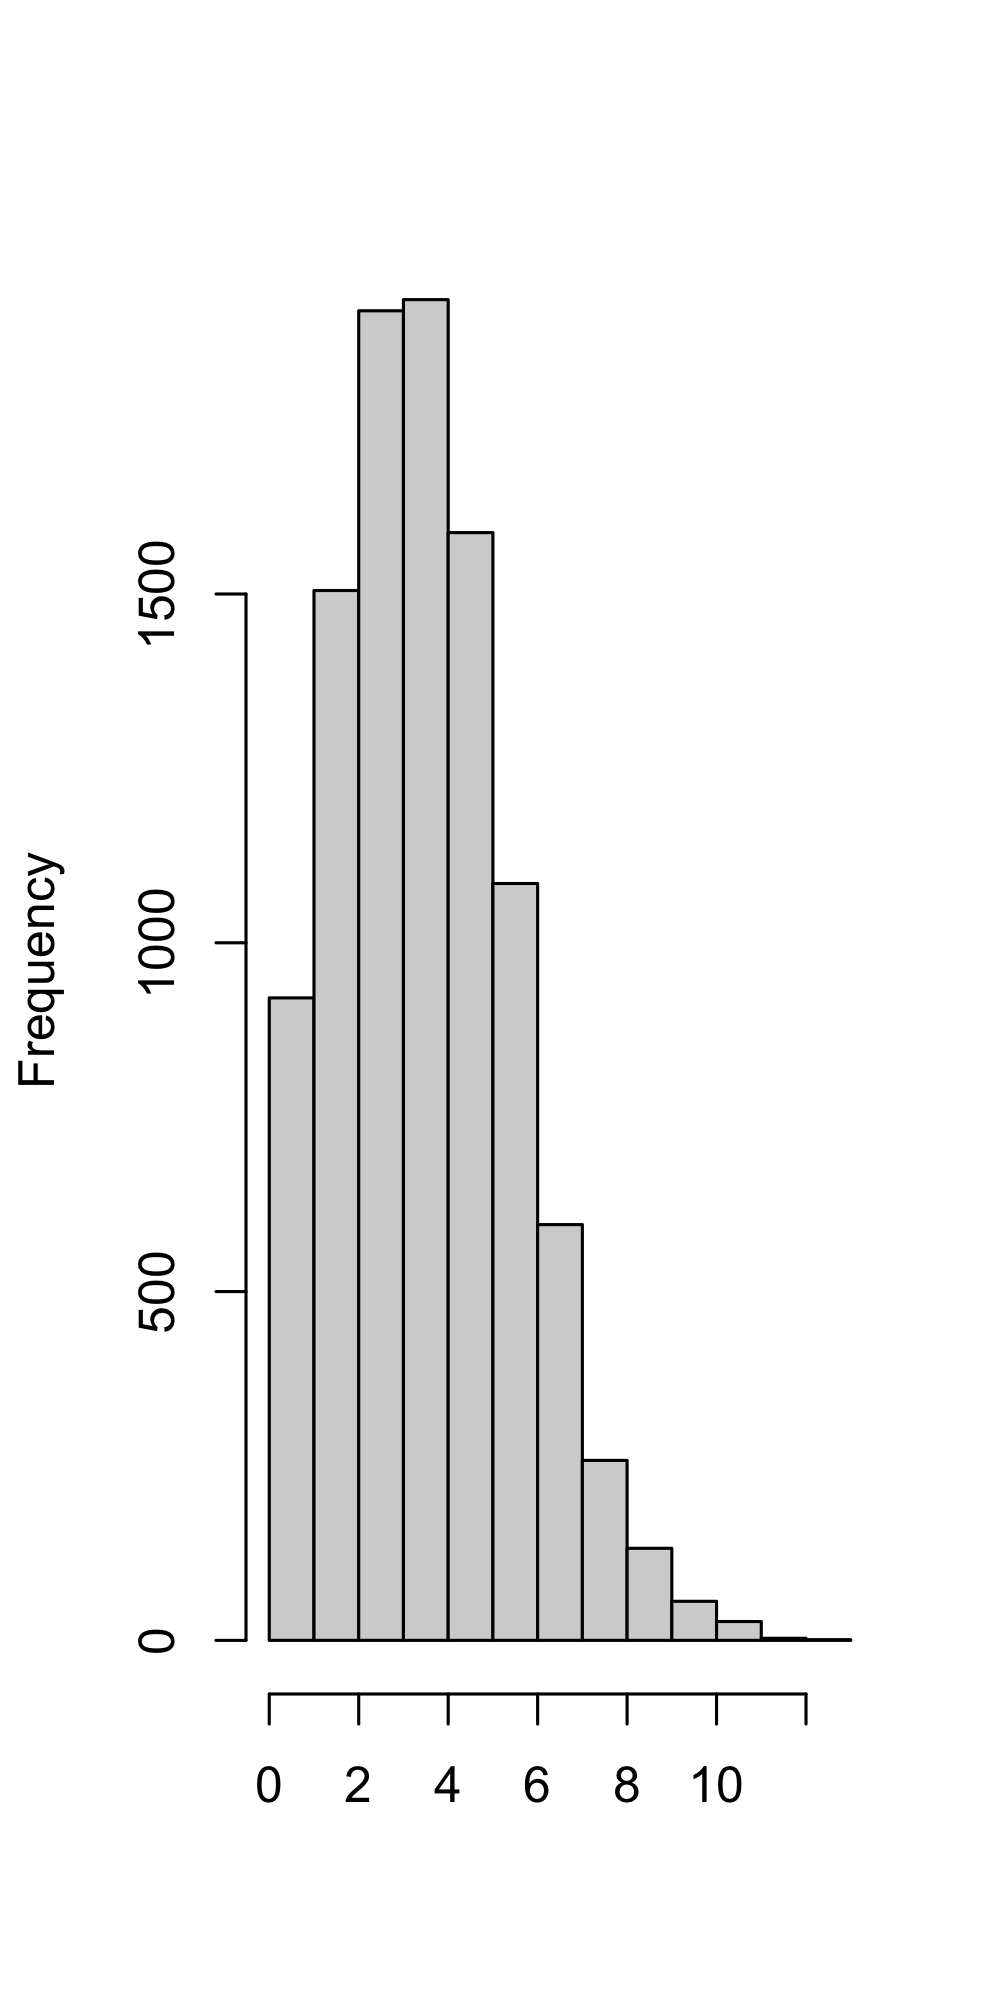
\includegraphics[width=1\linewidth]{E4_distpois.png}  
  \caption{Histogram of \texttt{rpois}(10000, 4).}
  \label{subfig1-1}
\end{subfigure}
\begin{subfigure}{.33\textwidth}
  \centering
  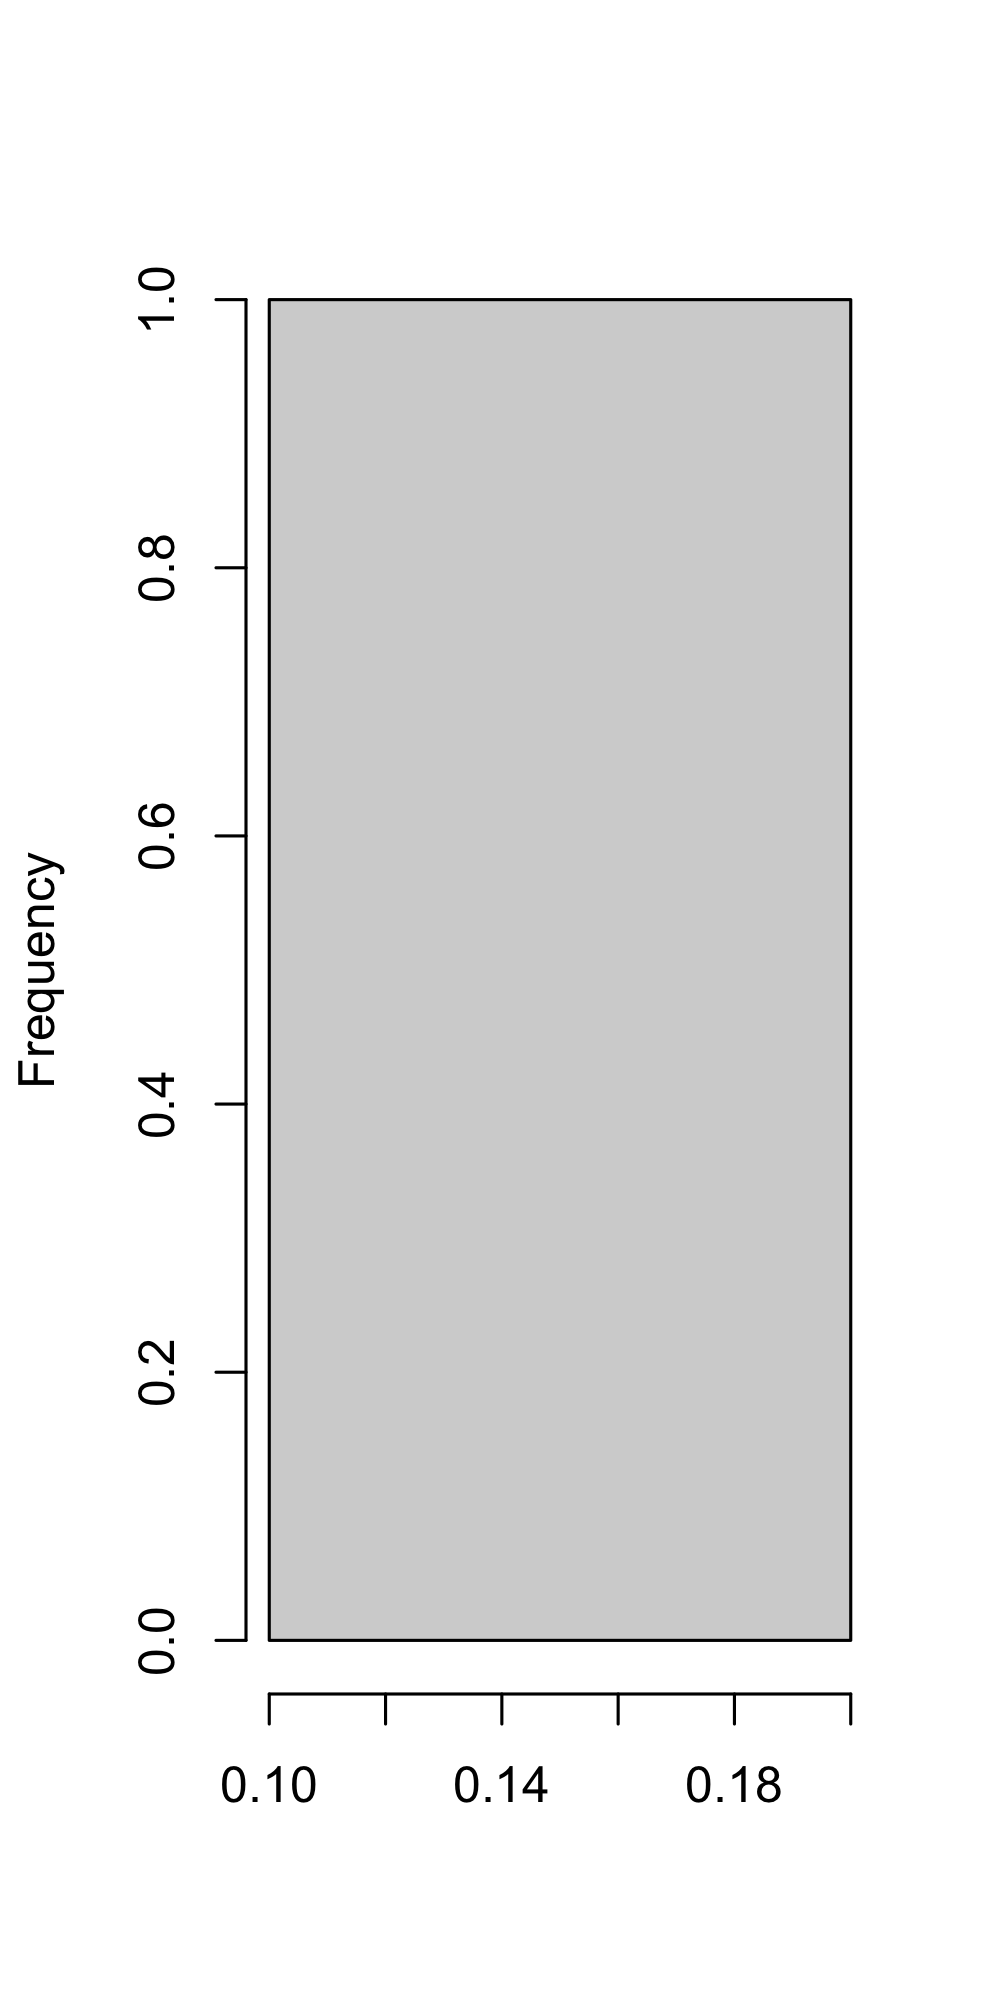
\includegraphics[width=1\linewidth]{E4_distexp.png}  
  \caption{Histogram of \texttt{rexp}(1, 4)}
  \label{subfig1-2}
\end{subfigure}
\begin{subfigure}{.33\textwidth}
  \centering
  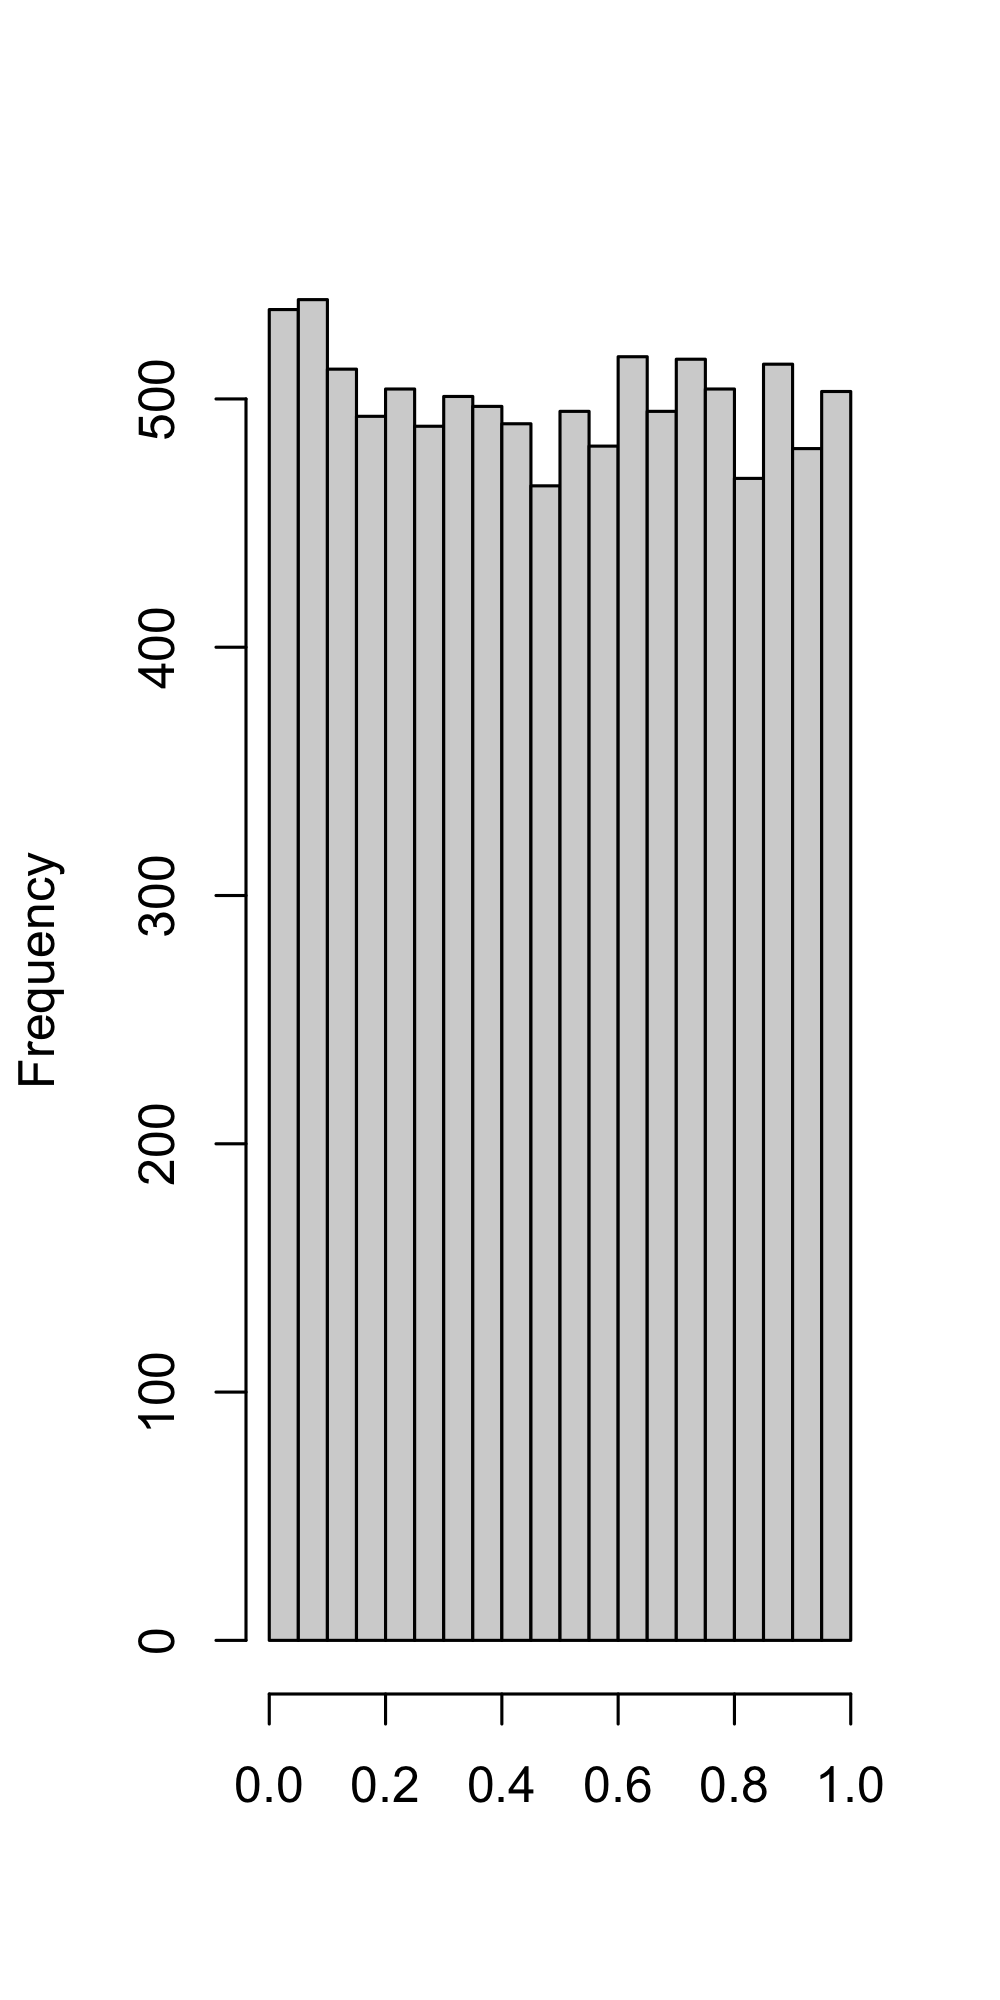
\includegraphics[width=1\linewidth]{E4_distunif.png}  
  \caption{Histogram of \texttt{runif}(10000)}
  \label{subfig1-3}
\end{subfigure}
\caption{Histograms showing the behaviours of each distribution (Poisson, Exponential and Uniform).}
\label{fig1}
\end{figure}


In order to search for ways to make them behave in a similar manner, we first needed an example of how the Poisson distribution works. Say we live near an airport, and we can see as an average, 4 planes in the span of one hour. Now as an experiment we record the number of planes we see every hour for 10,000 hours. In Subfigure \ref{subfig1-1} we can see such behaviour. As expected, the majority of the plane occurrences are 3, 4 or 5 inside the interval of an hour. There is a better chance of no planes showing than there is to have more than 7 in this interval. Understanding this, we begin now to translate this performance to the exponential and uniform distributions \cite{randvariates}.\\

For the Poisson distribution it is possible to develop several generators that help us make a simply uniformly fast Poisson distribution. Such generators can be classified in several groups:

\begin{enumerate}
\item Generators that are based on the connection with homogeneous Poisson process. \cite{atkinson1979computer}. These type of generators are simple and run in expected time proportional to $\lambda$.
\item Inversion methods, that use sequential search starting at 0 and run in expected time proportional to $\lambda$. If the sequential search starts here, the expected time is $\mathcal{O} (\sqrt{\lambda})$ \cite{kemp1990new}
\item Generators that are based on recursive properties of the distribution.
\item Rejection methods.
\item The acceptance complement method with the normal distribution as a starting distribution.
\end{enumerate}

\smallskip

In this case, one of the simple generators we have the exponential and uniform distribution. Beginning with the connection between the Poisson distribution and exponential arrival times in a homogeneous point process we have the Lemma \ref{lema1} for the Poisson distribution \cite{randvariates}.\\

\begin{lemma}\label{lema1}
If $E_1, E_2, ...$ are exponential random variables, and $X$ is the smallest integer such that \\
\begin{equation*}
\sum_{i=1}^{X+1}E_i>\lambda
\end{equation*}
then $X$ is Poisson ($\lambda$).
\end{lemma}

As proof of this Lemma \ref{lema1} we are presented with Proof \ref{prof1}:
\begin{proof}\label{prof1}
Let $f_k$ be the gamma (k) density. 
\begin{equation*}
P(X\leq k) = P (\sum_{i=1}^{k+1}E_i>\lambda) = \int_{\lambda}^\infty f_{k+1}(y)dy
\end{equation*}
Thus, by partial integration,
\begin{align*}
P(X=k) &= P (X \leq k ) - P (X\leq k-1) \\
&=\int_\lambda^\infty(f_{k+1}(y) - f_k (y)) dy\\
&=\int_\lambda^\infty(y-k) \frac{y^{k-1}}{k!} e^{-y} dy\\
&=\frac{1}{k!} \int_\lambda^\infty d(-y^k e^{-y})\\
&= e^{-\lambda} \frac{\lambda^k}{k!}.
\end{align*}
\end{proof}


In the end of this proof we see the same equation as we explained in the introduction in Equation \ref{eq1} on the Poisson distribution. The algorithm that was based upon this proof
is shown in Algorithm \ref{alg1}:\\

\begin{algorithm}[]
X $\leftarrow$ 0\;
Sum $\leftarrow$ 0\;
 \While{TRUE}{
  Generate an exponential random variate E\;
  Sum $\leftarrow$ Sum $+$ E\;
  \eIf{Sum $< \lambda$}{
   X $\leftarrow$ X $+$ 1\;
   }{
   RETURN X\;
  }
 }
 \caption{Poisson generator based upon exponential inter-arrival times}\label{alg1}
\end{algorithm}

\smallskip

If we translate this to the example of the planes, we randomly generate 10,000 distributed random variables X, interpreting X as the waiting time from the passing of one plane to another measured by the hour. If we know the value of $\lambda$ is 4 as the average of planes, the time that each event happens can be obtained from the cumulative sum of the waiting times from event to event.  We can then aggregate the number of events that happen per unit time, and make an histogram out of them. \\

Remembering the information of \texttt{R help} we put as a parameter the $\lambda$ and not $1/\lambda$. Using the same parameters as the Poisson example we now have the results shown in Figure \ref{fig2}. Further analysis of both Subfigures \ref{subfig2-1} and \ref{subfig2-2} we can see that the behavior is very similar, in contrast with the first experimentation in Subfigure \ref{subfig1-2}

\begin{figure}[]
\begin{subfigure}{.5\textwidth}
  \centering
  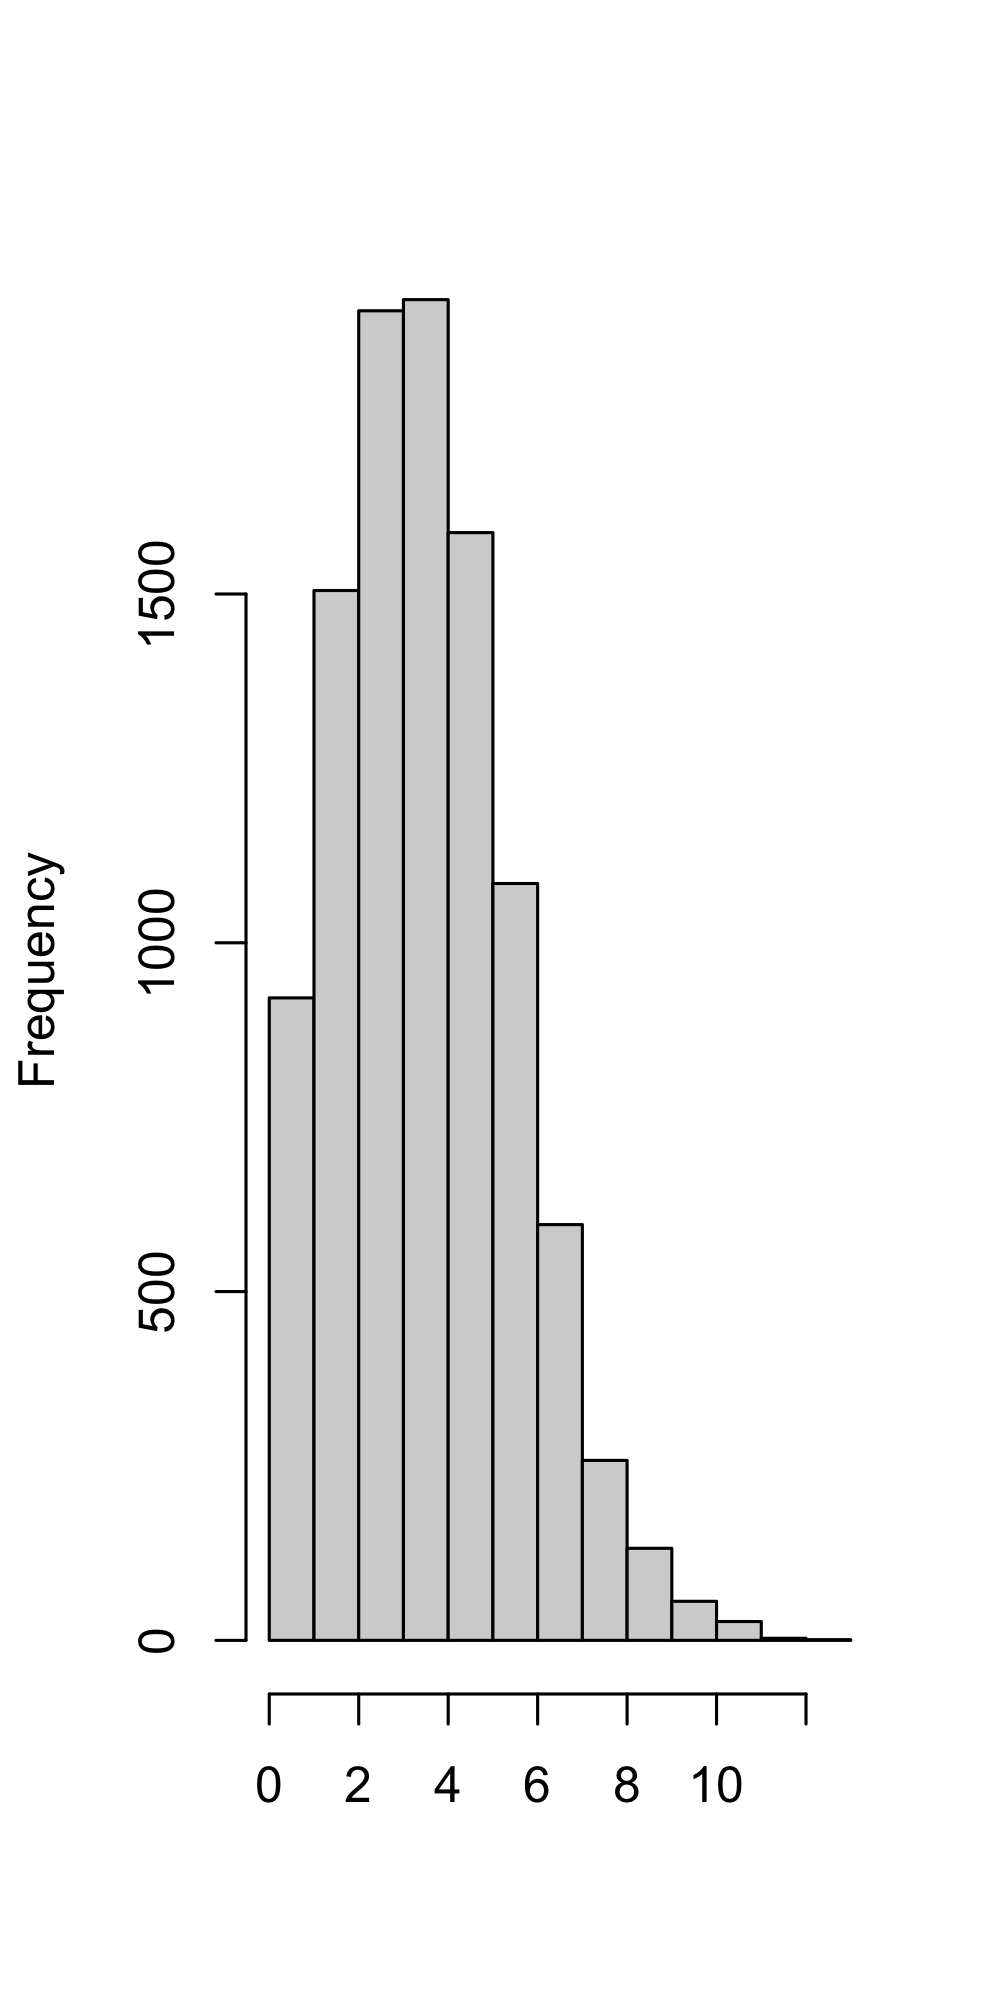
\includegraphics[width=1\linewidth]{E4_distpois.png}  
  \caption{Histogram of \texttt{rpois}(10000, 4).}
  \label{subfig2-1}
\end{subfigure}
\begin{subfigure}{.5\textwidth}
  \centering
  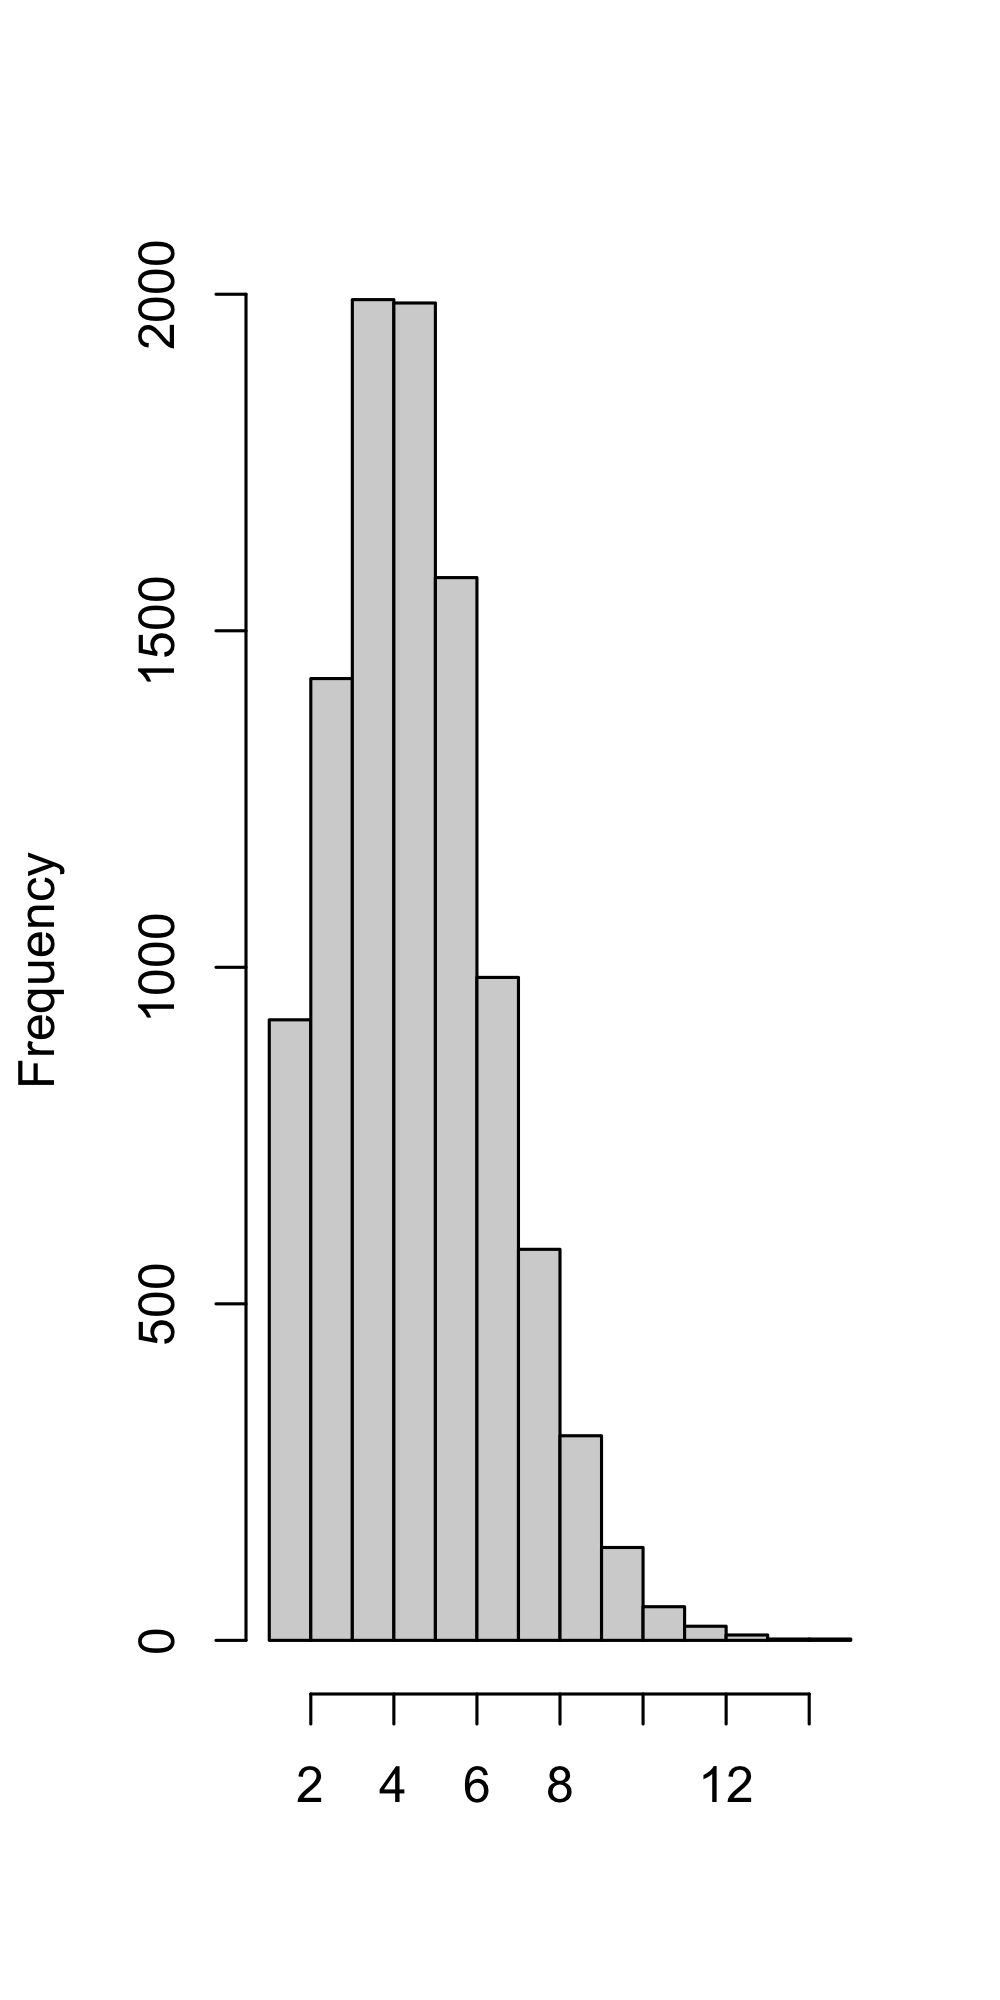
\includegraphics[width=1\linewidth]{E4_exponencial.png}  
  \caption{Histogram of experimentation with cumulative sum of \texttt{rexp}}
  \label{subfig2-2}
\end{subfigure}
\caption{Histograms showing the behaviour of distribution Poisson and cumulative exponential experimentation.}
\label{fig2}
\end{figure}

\clearpage


For the uniform distribution we take on the fact that a uniform random variable is distributed as $e^{-E}$, we can equate the Lemma \ref{lema1} to the next Lemma \ref{lema2} \cite{randvariates}.

\begin{lemma}\label{lema2}
Let $U_1, U_2, ...$ be uniform $[0,1]$ random variables, and $X$ is the smallest integer such that \\
\begin{equation*}
\prod_{i=1}^{X+1}U_i <e^{-\lambda}
\end{equation*}
then $X$ is Poisson ($\lambda$).
\end{lemma}

The resulting algorithm of this Lemma is equivalent as Algorithm \ref{alg1}

\begin{algorithm}[]
X $\leftarrow$ 0\;
Prod $\leftarrow$ 1\;
 \While{TRUE}{
  Generate a uniform $[0,1]$ random variate U\;
  Prod $\leftarrow$ Prod U\;
  \eIf{Prod $>e^{-\lambda}$ (the constant should be computed only once) } {
   X $\leftarrow$ X $+$ 1\;
   }{
   RETURN X\;
  }
 }
 \caption{Poisson generator based upon multiplication of uniform random variates.}\label{alg2}
\end{algorithm}

\begin{figure}[]
\begin{subfigure}{.5\textwidth}
  \centering
  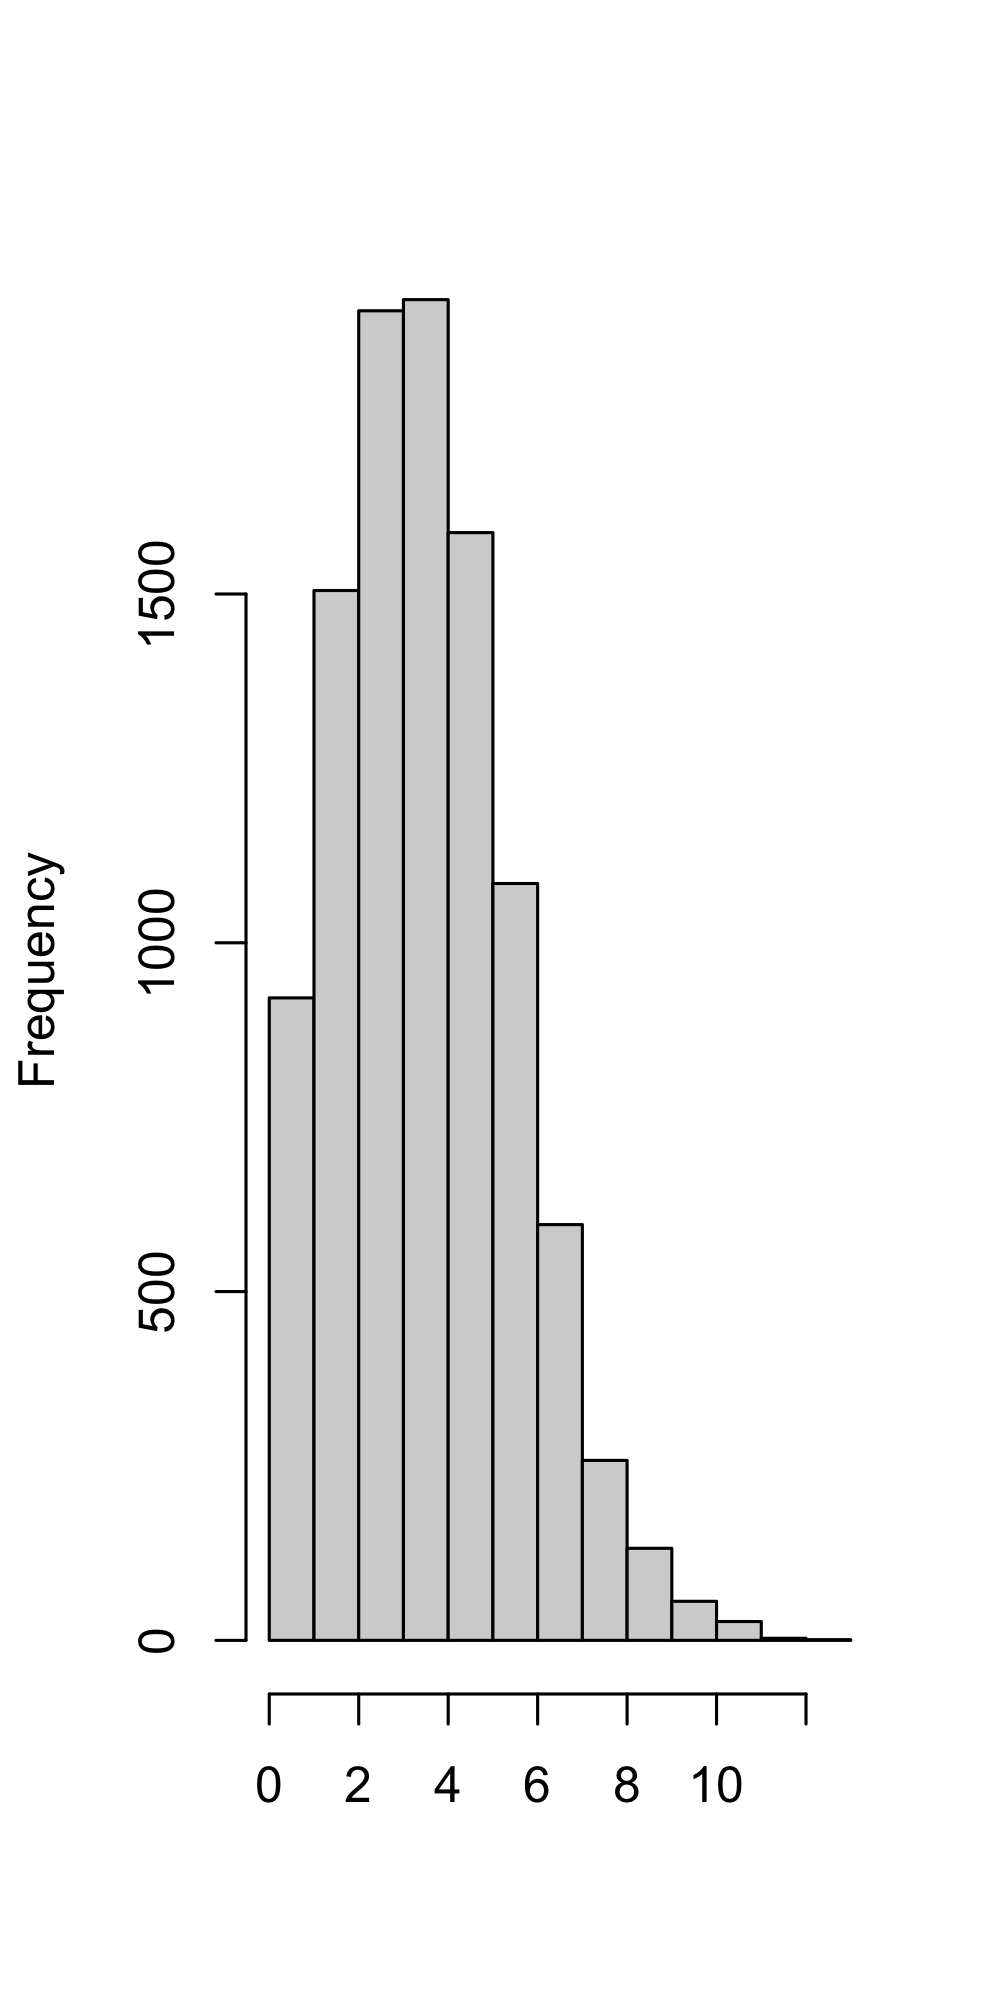
\includegraphics[width=1\linewidth]{E4_distpois.png}  
  \caption{Histogram of \texttt{rpois}(10000, 4).}
  \label{subfig3-1}
\end{subfigure}
\begin{subfigure}{.5\textwidth}
  \centering
  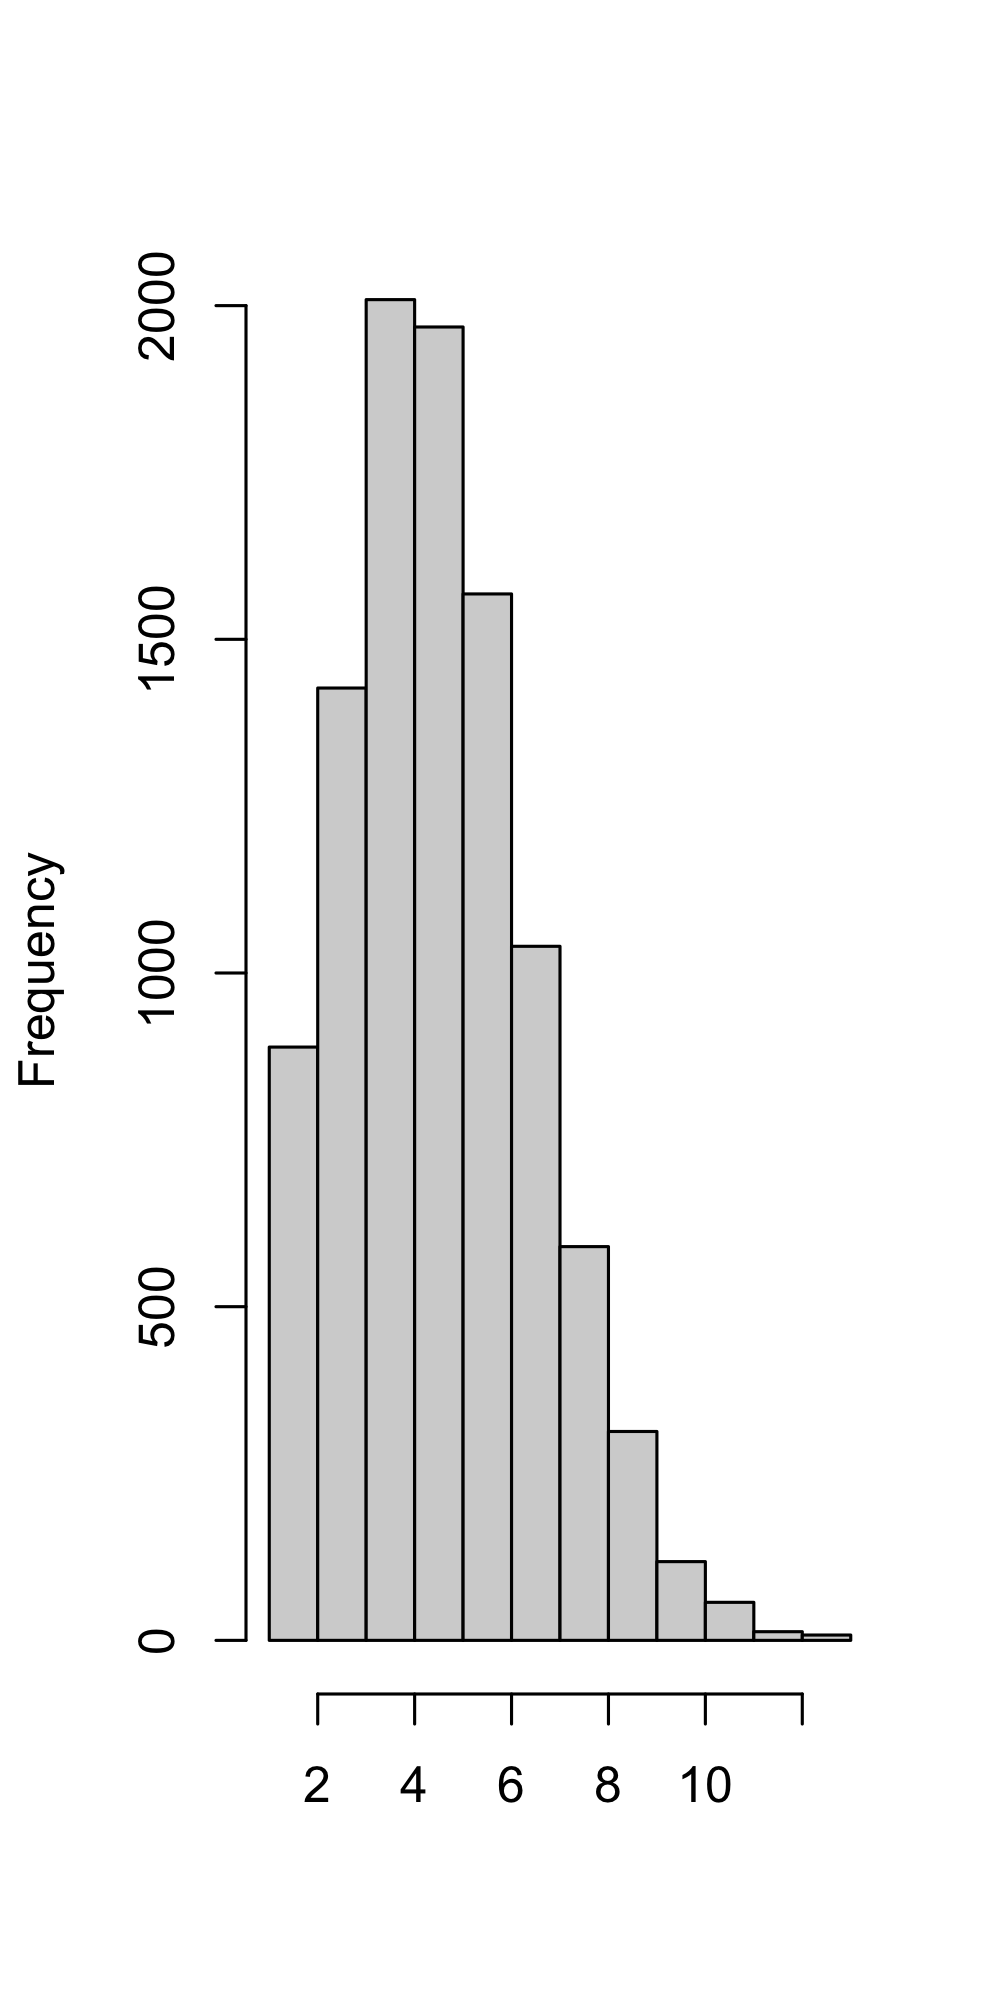
\includegraphics[width=1\linewidth]{E4_uniforme.png}  
  \caption{Histogram of experimentation with multiplication of uniform random variates \texttt{runif}}
  \label{subfig3-2}
\end{subfigure}
\caption{Histograms showing the behaviours of distribution poisson and uniform random variates experimentation.}
\label{fig3}
\end{figure}

\clearpage

In this case, the experiment of the planes was not so clear in mind, because the involvement of the exponential part in the code did not make much sense. So we went to the \texttt{R} code to see what was the result of each of the experiments, exponential and uniform. \\

We printed the last iteration of each distribution, and in the case of the exponential, the cumulative sum was clear, as the results were 0.0614 and 1.4261. If the goal set is 1, those two events were enough to complete the interval. In the case of the uniform distribution the last iteration numbers where 0.2350, 0.8153, 0.4806, and 0.0748. At first this did not make sense, but after calculating the product of all this numbers and comparing them to the result of $1/-\lambda$ it made sense why we had to use multiplication instead of cumulative sum. \\

\section{Experimentation with different parameters}

In Figure \ref{fig5} there we can see all the distributions in different parameters. It is very curious that the lowest parameter on lambda in all three different iterations of Subfigures \ref{subfig5-1}, \ref{subfig5-2} and \ref{subfig5-3}, they all show a behaviour similar to the exponential that we saw in the introduction of this work. Subfigures \ref{subfig5-4}, \ref{subfig5-5} and \ref{subfig5-6}, all with lambda = 5, resemble the Poisson distribution and Subfigures \ref{subfig5-7}, \ref{subfig5-8} and \ref{subfig5-9} with lambda = 10 to the normal distribution.\\

\begin{figure}[]
\begin{subfigure}{.33\textwidth}
  \centering
  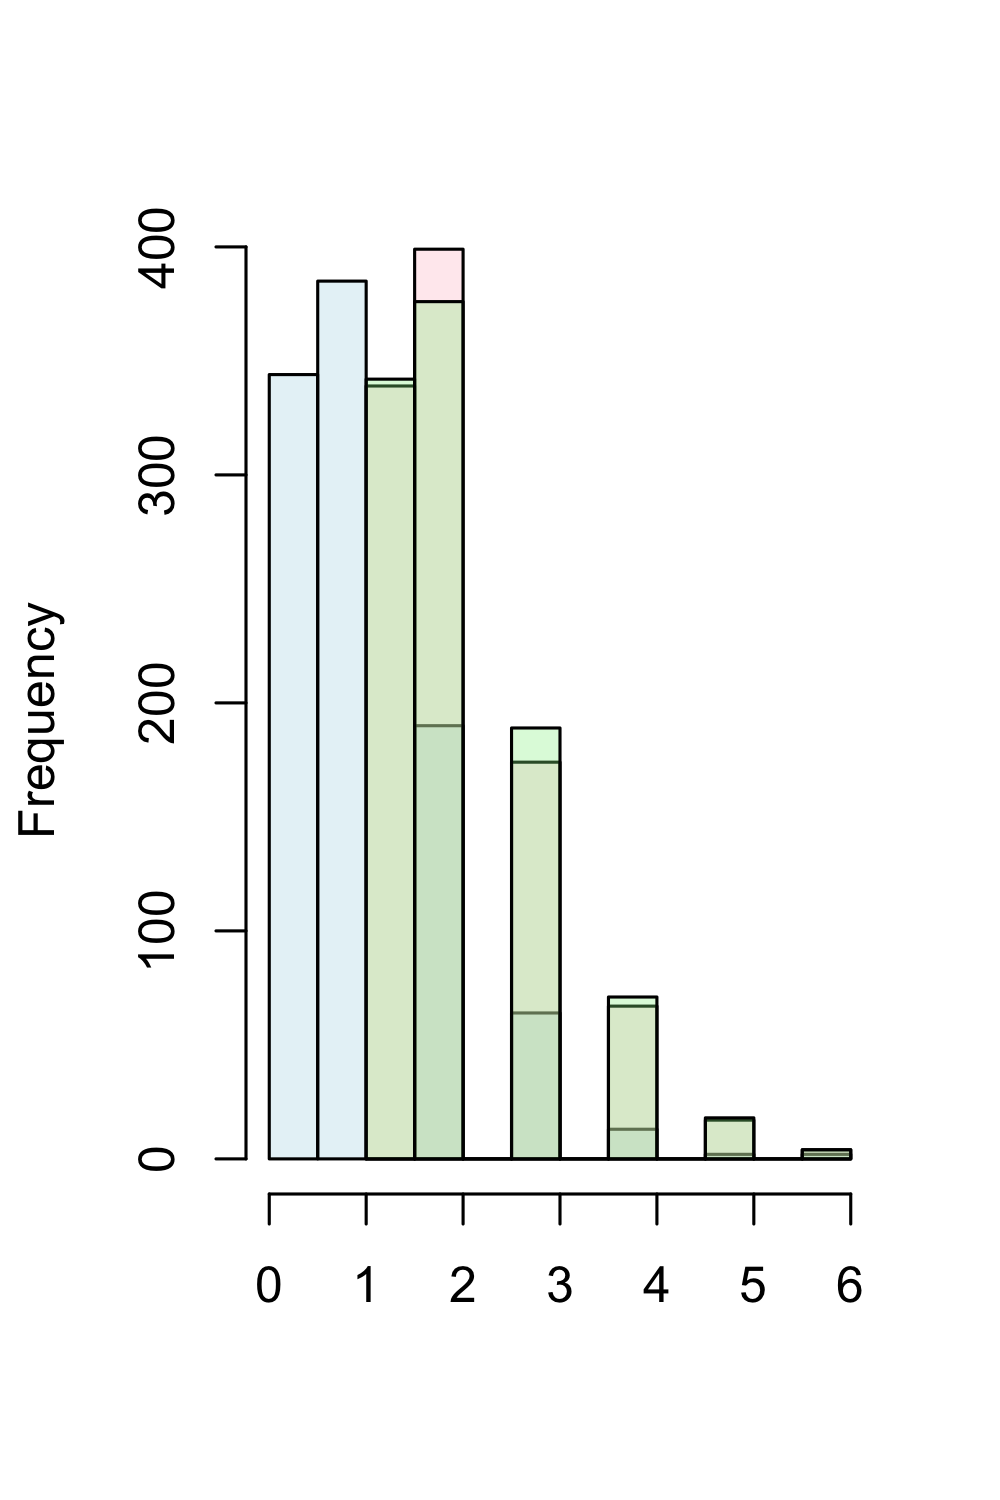
\includegraphics[width=.8\linewidth]{e4-1_1000.png}  
  \caption{$\lambda$ = 1, and replica = 1,000}
  \label{subfig5-1}
\end{subfigure}
\begin{subfigure}{.33\textwidth}
  \centering
  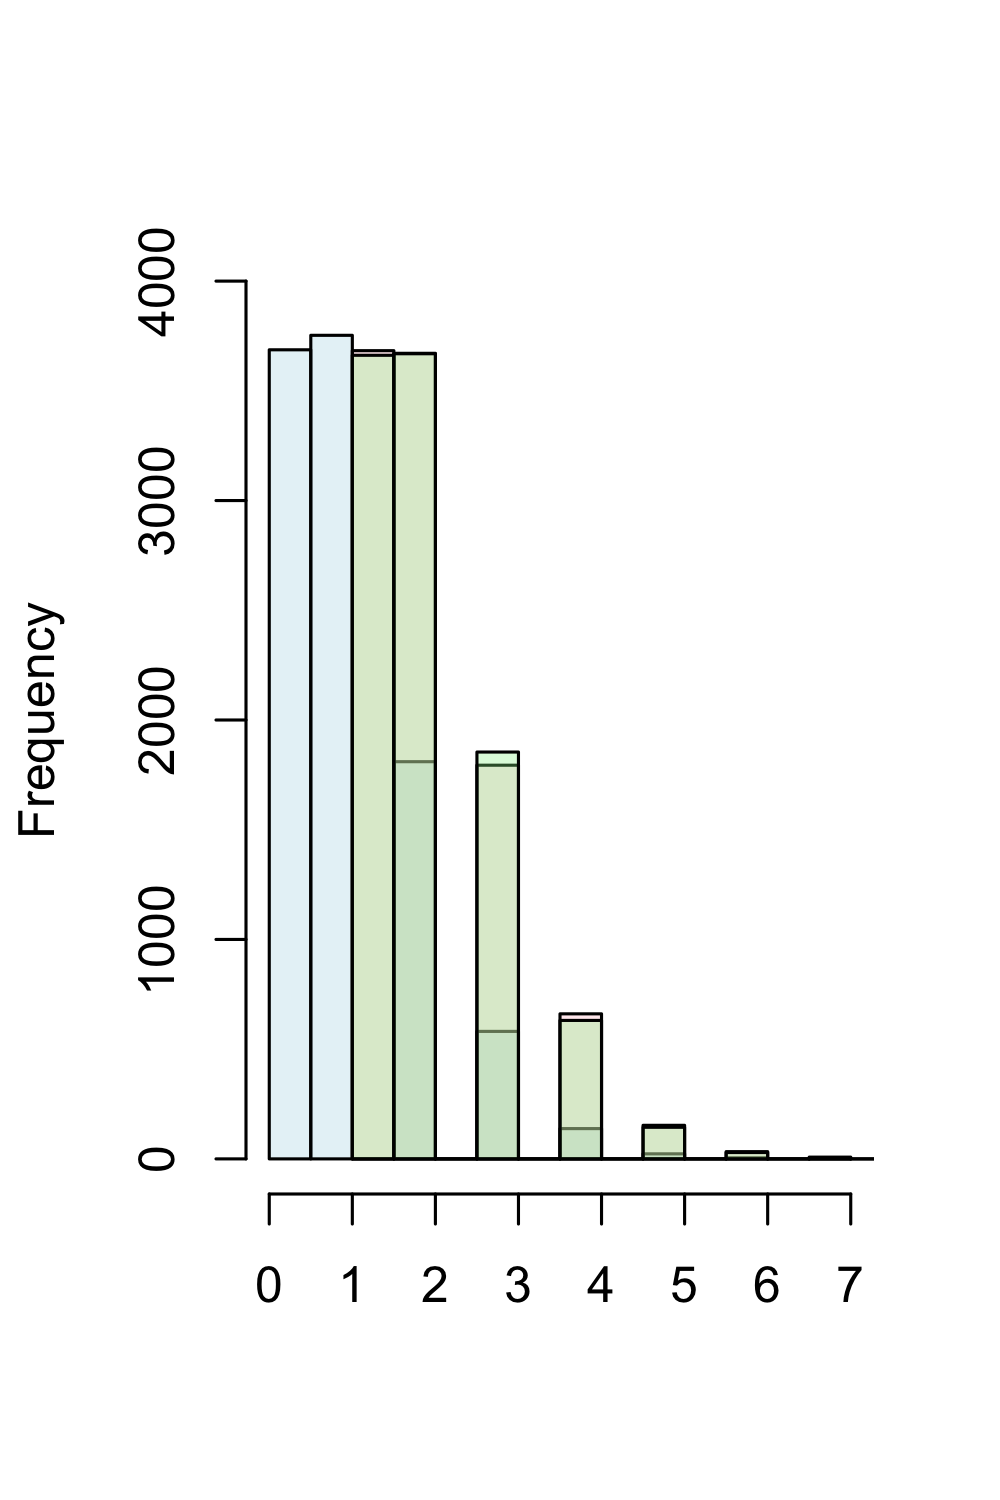
\includegraphics[width=.8\linewidth]{e4-1_10000.png}  
  \caption{$\lambda$ = 1, and replica = 10,000}
  \label{subfig5-2}
\end{subfigure}
\begin{subfigure}{.33\textwidth}
  \centering
  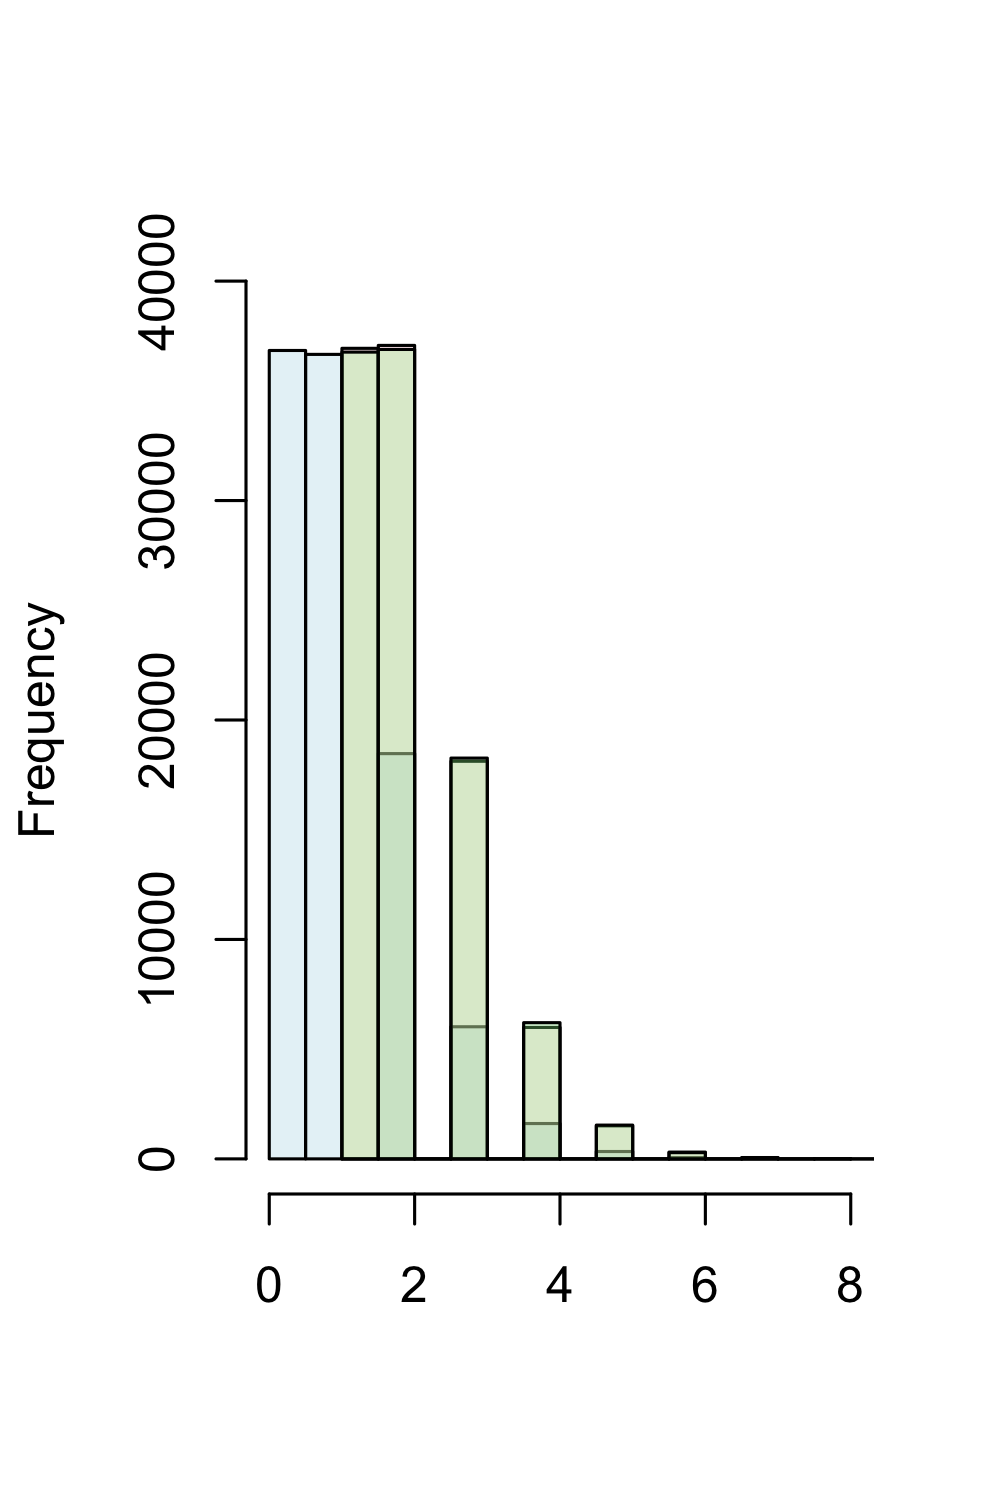
\includegraphics[width=.8\linewidth]{e4-1_100000.png}  
  \caption{ $\lambda$ = 1, and replica = 100,000}
  \label{subfig5-3}
\end{subfigure}
\newline
\begin{subfigure}{.33\textwidth}
  \centering
  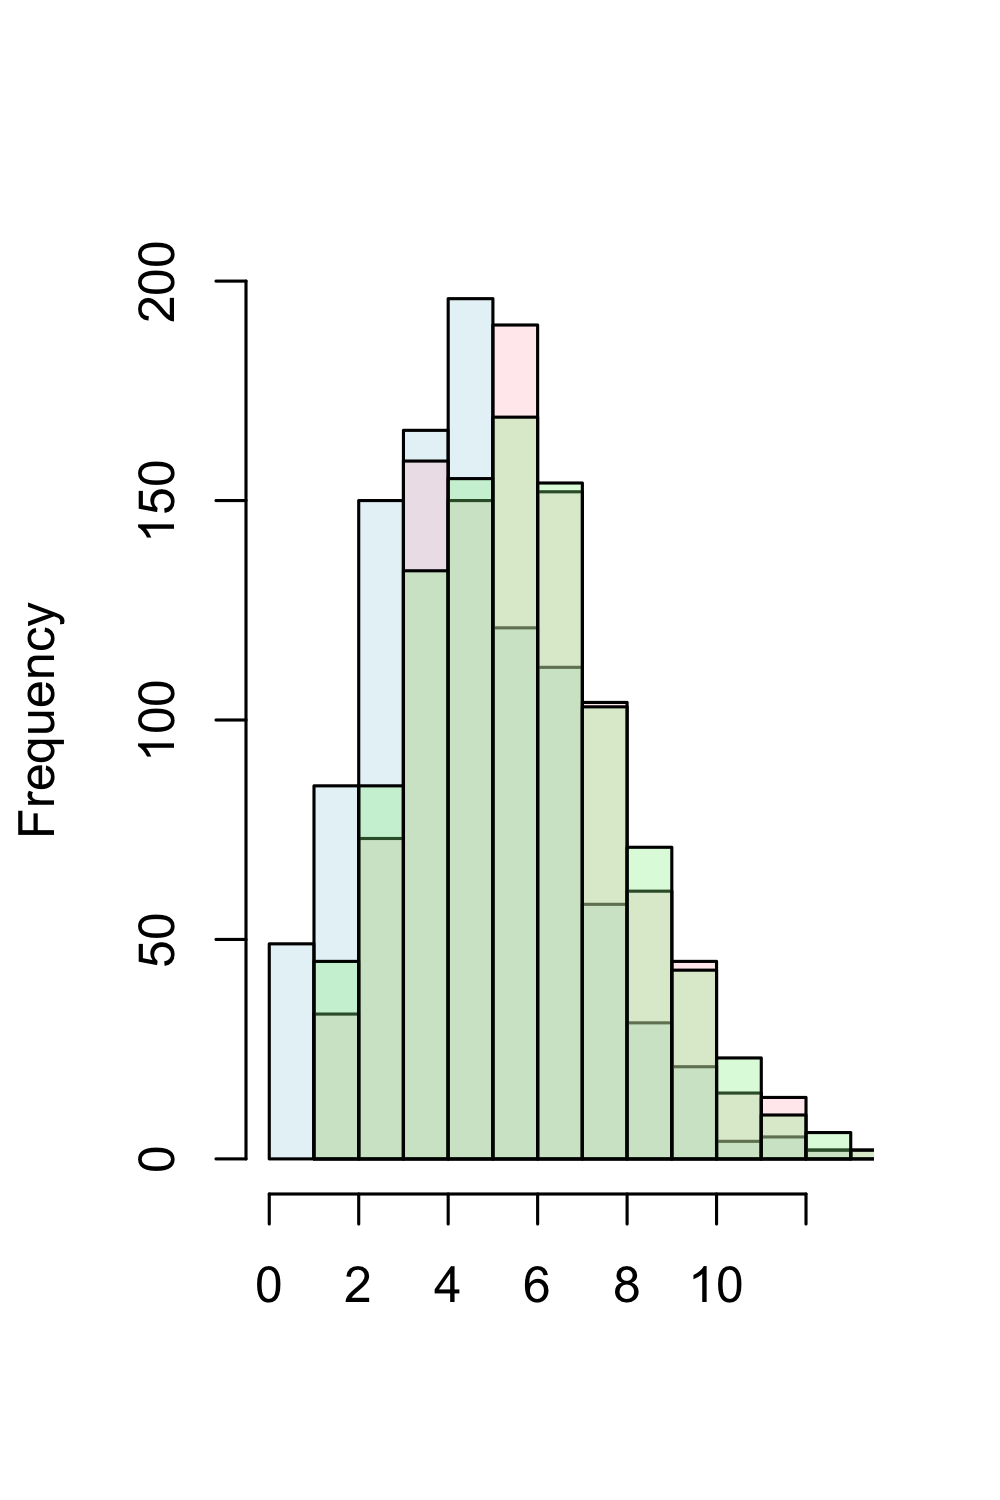
\includegraphics[width=.8\linewidth]{e4-5_1000.png}  
  \caption{$\lambda$ = 5, and replica = 1,000}
  \label{subfig5-4}
\end{subfigure}
\begin{subfigure}{.33\textwidth}
  \centering
  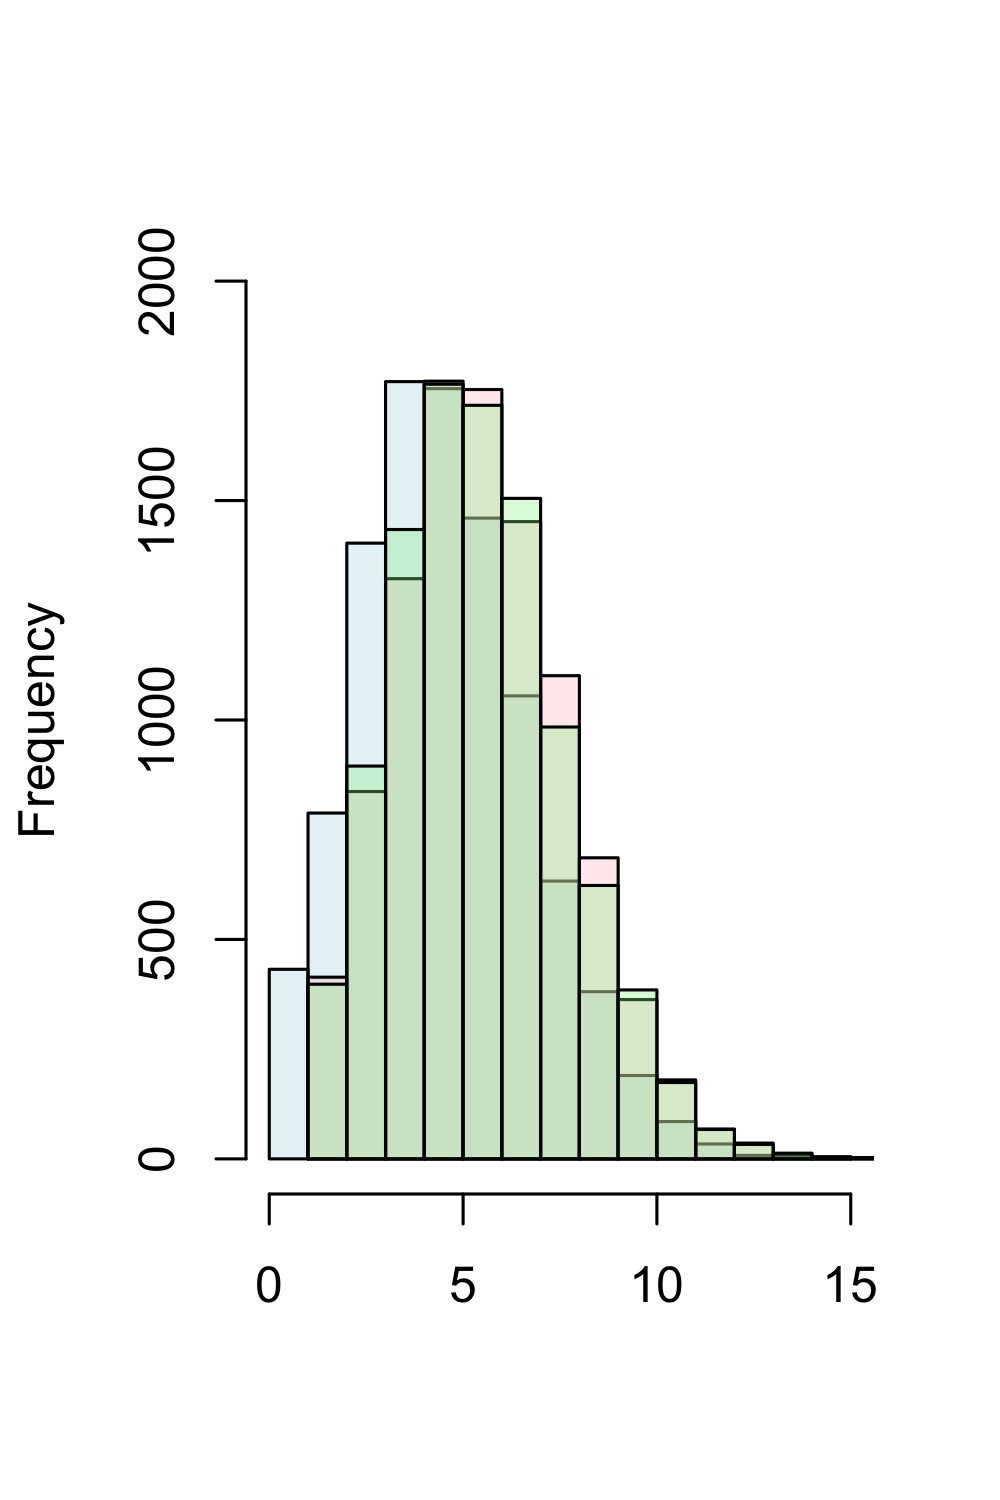
\includegraphics[width=.8\linewidth]{e4-5_10000.png}  
  \caption{$\lambda$ = 5, and replica = 10,000}
  \label{subfig5-5}
\end{subfigure}
\begin{subfigure}{.33\textwidth}
  \centering
  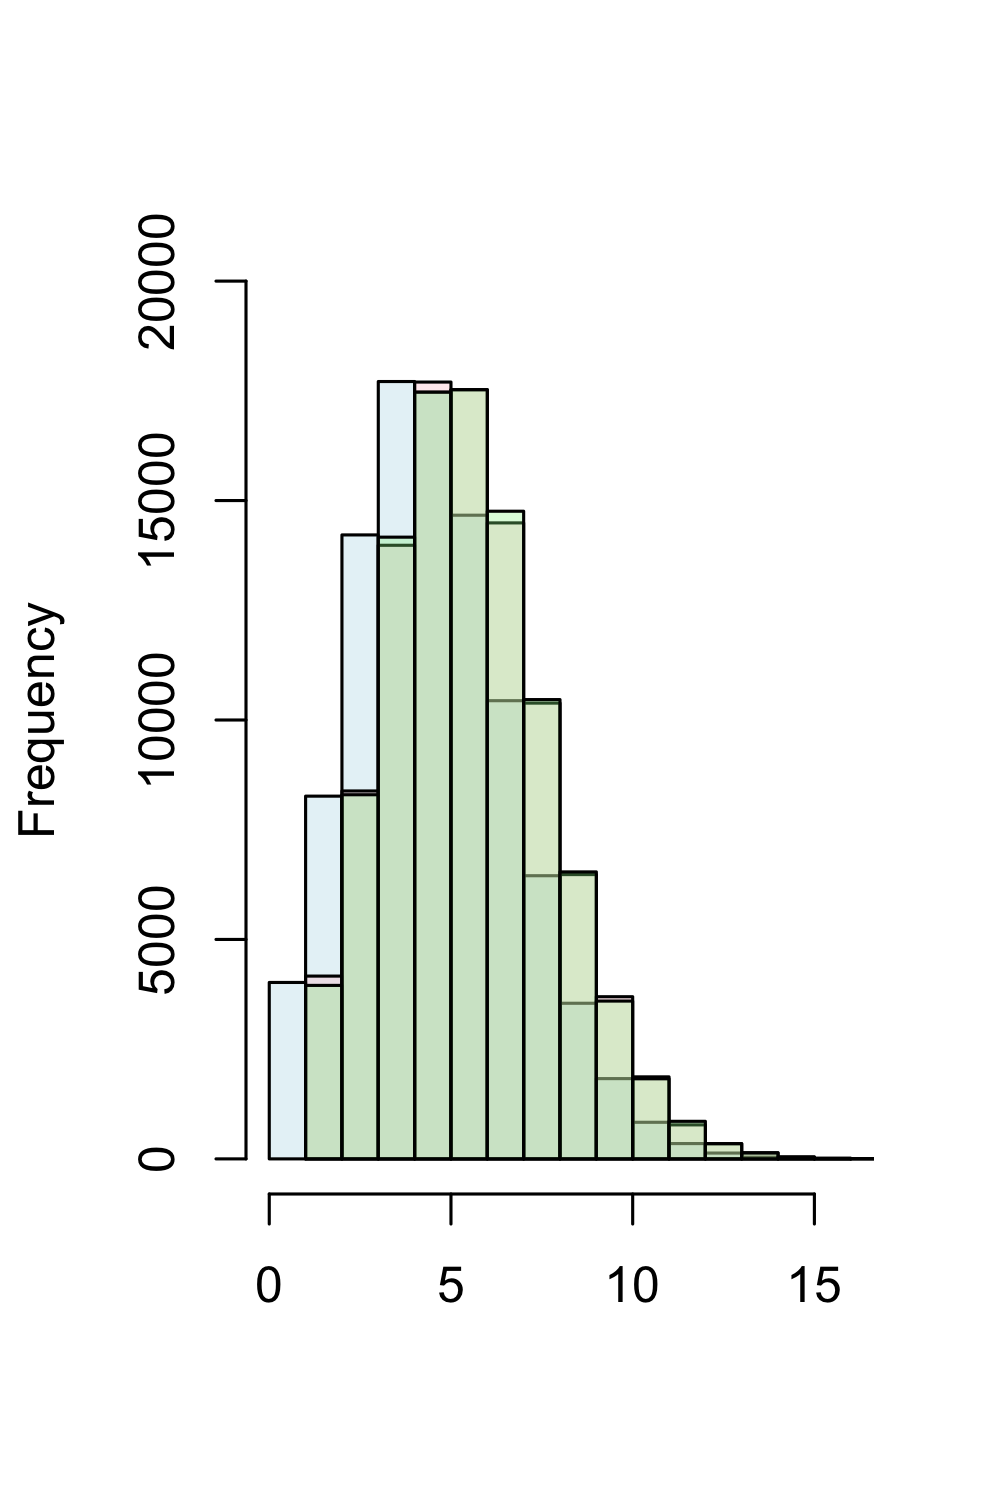
\includegraphics[width=.8\linewidth]{e4-5_100000.png}  
  \caption{$\lambda$ = 5, and replica = 100,000}
  \label{subfig5-6}
\end{subfigure}
\newline
\begin{subfigure}{.33\textwidth}
  \centering
  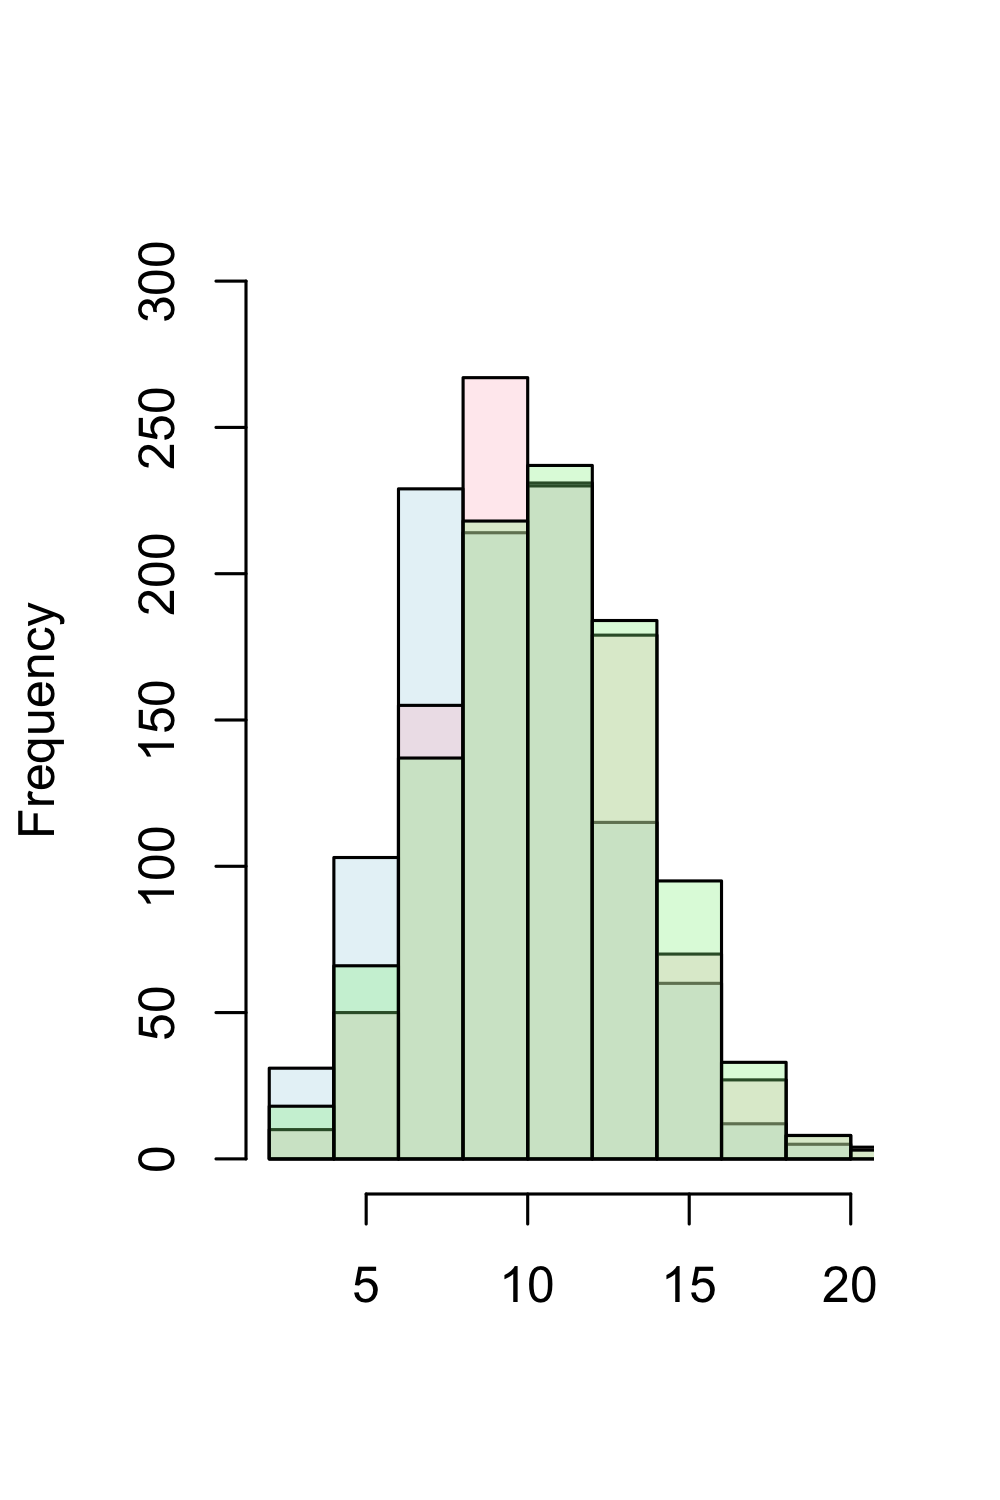
\includegraphics[width=.8\linewidth]{e4-10_1000.png}  
  \caption{$\lambda$ = 10, and replica = 1,000}
  \label{subfig5-7}
\end{subfigure}
\begin{subfigure}{.33\textwidth}
  \centering
  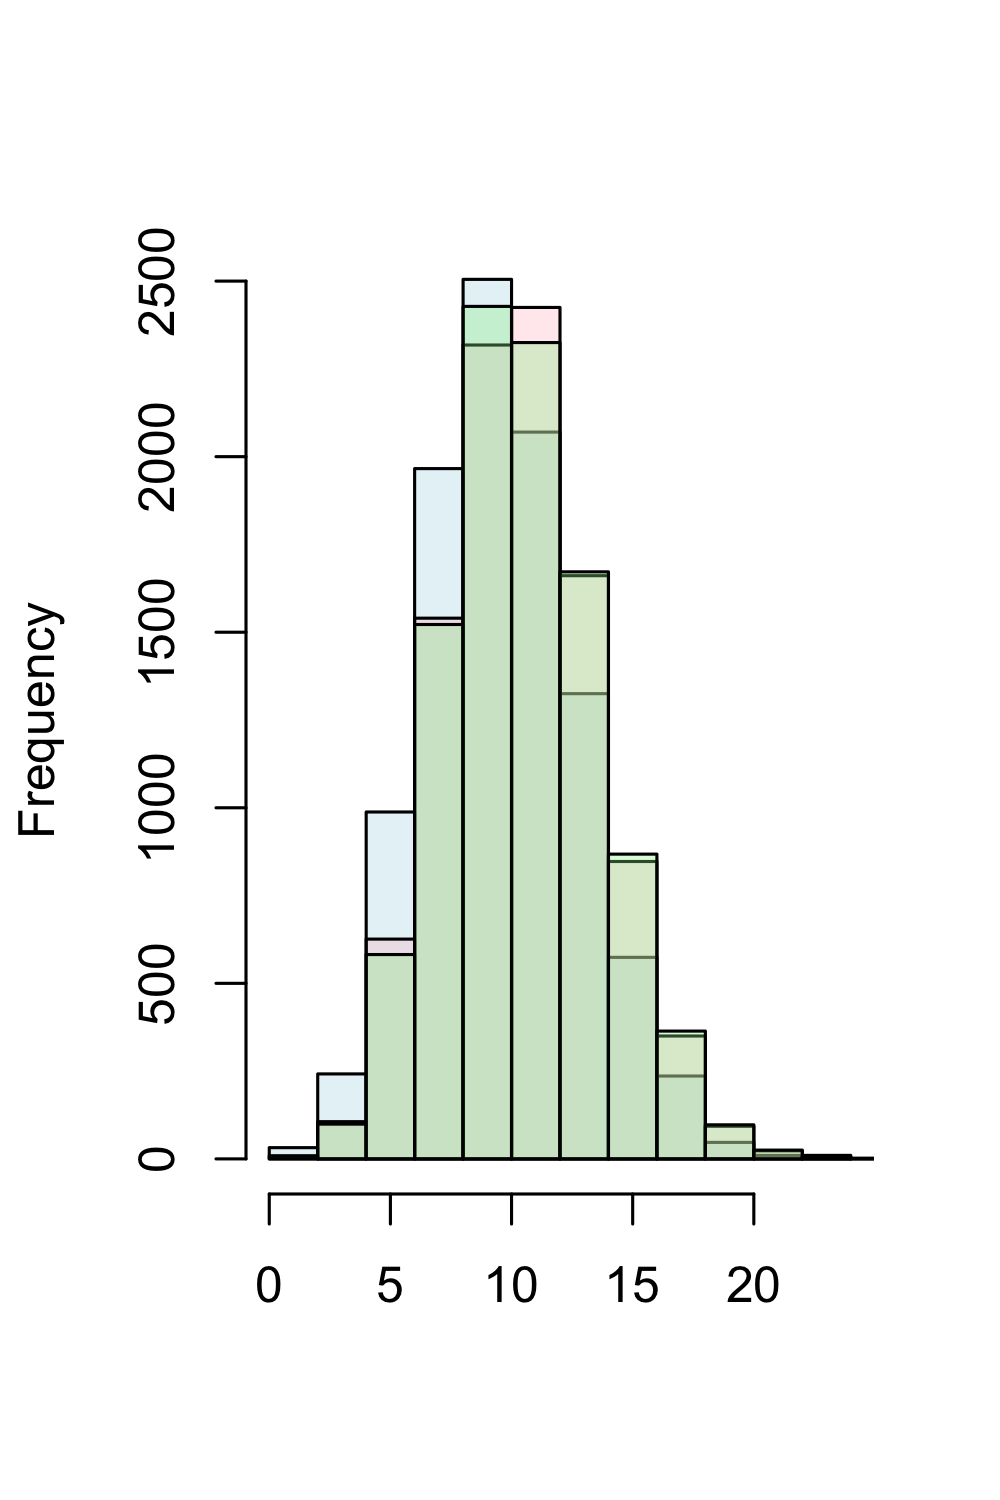
\includegraphics[width=.8\linewidth]{e4-10_10000.png}  
  \caption{$\lambda$ = 10, and replica = 10,000}
  \label{subfig5-8}
\end{subfigure}
\begin{subfigure}{.33\textwidth}
  \centering
  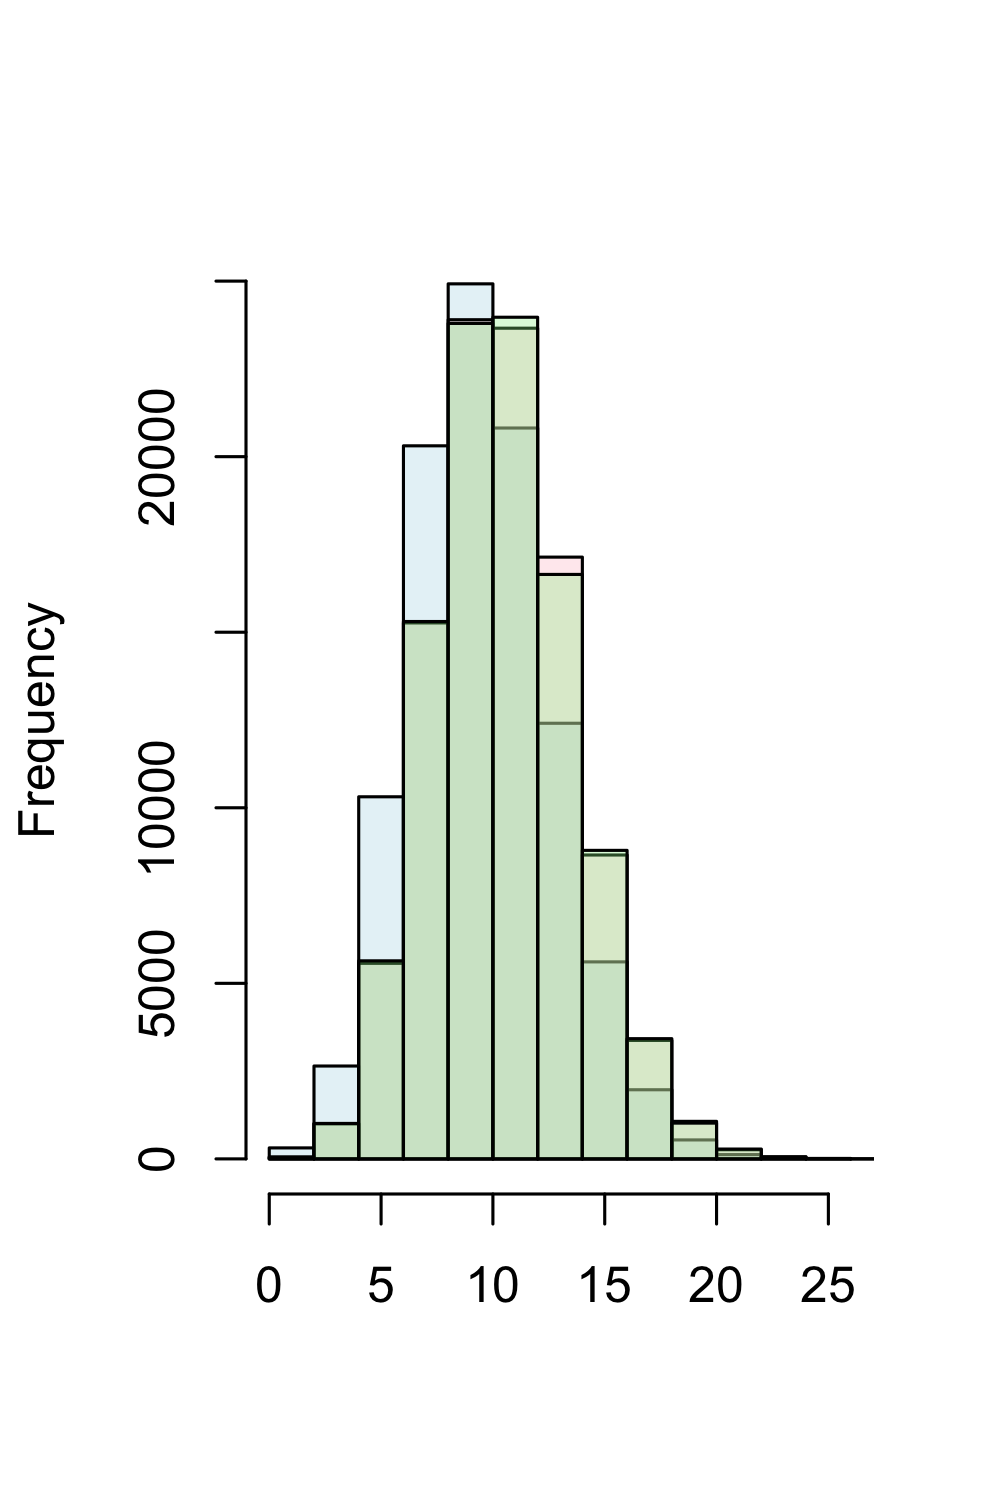
\includegraphics[width=.8\linewidth]{e4-10_100000.png}  
  \caption{$\lambda$ = 10, and replica = 100,000}
  \label{subfig5-9}
\end{subfigure}
\caption{Histograms of all the distributions with different parameters. The blue represents the Poisson distribution, the pink is the exponential distribution, and the green the uniform distribution. }
\label{fig5}
\end{figure}




\clearpage
\section{Conclusions}

The conclusions arrived in this practice where more clear in the exact order we mentioned them. Seeing the Poisson distribution first as an example made easier to understand. Then to transform the exponential distribution to the behaviour of the Poisson one was easy because the concept of cumulative sum as depicted on the Figure \ref{figelisa} Dr. Elisa gave us in class was simple. After all of that, the uniform distribution using multiplication to lower the final result to fit inside the exponential condition was a bit harder to understand, but the experimentation in \texttt{R} made it easier to visualize and digest.\\

Figure \ref{fig5} is also something interesting, how changing the parameters of lambda, we can change the behaviour of the distribution, making it seem like other distributions.\\

\begin{figure}[]
  \centering
  
\includegraphics[width=1\linewidth]{intervals.png}  
  \caption{Example made by Dr. Elisa as a visual aid of how the Poisson distribution works.}
  \label{figelisa}
\end{figure}


\bibliographystyle{plainnat}
\bibliography{tarea4}


 
\end{document}